\documentclass[xcolor=dvipsnames]{beamer} 
\usepackage[french]{babel}
\usepackage[utf8]{inputenc}
\usepackage{graphics}
\usepackage{tikz}
\usecolortheme[named=OliveGreen]{structure} 
\useoutertheme{infolines}
\usetheme[height=7mm]{Berkeley}
\setbeamertemplate{blocks}[rounded][shadow=true] 
\setbeamertemplate{navigation symbols}{} 
\setbeamertemplate{footline}[page number]{}
\author{Lorenzo Fundaró (06-39559)\\ José Garrido (06-39590)} 
\title{Information Retrieval \\vs. \\Information Extraction} 
\institute{Universidad Simón Bolívar\\Inteligencia Artificial 2} 

\begin{document}

\begin{frame}
\titlepage
\end{frame}


\begin{frame}
\frametitle{Information Extraction - Introducción}
\begin{itemize}
 \item \textbf{Text Understanding}: \emph{El complemento de Information Retrieval}. Semántica en oraciones, inferencias implícitas, complejidad lingüística.
 \item Information Extraction se encuentra en la zona intermedia entre Information Retrieval y Text Understanding.
\end{itemize}
\begin{center}
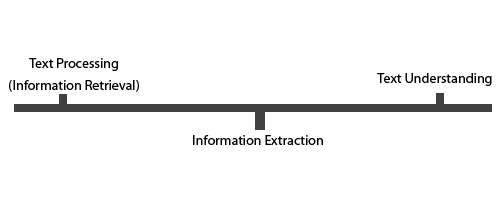
\includegraphics[scale=0.4]{IEandIR.png}
\end{center}
\end{frame}

\begin{frame}
\frametitle{Information Extraction - Definición}
\begin{itemize}
 \item El área de Information Extraction se caracteriza por \textbf{extraer desde diferentes fuentes secciones de datos y hechos relevantes para representarlos de alguna manera útil}.
 \item Message Understanding Conferences (MUC): Principal influencia en el área de Information Extraction. Evolución, historia, competencias, problemas de IE.
\end{itemize}
\end{frame}


\begin{frame}
\frametitle{Information Extraction - Ejemplo}
\begin{itemize}
 \item Texto con noticia de ataque terrorista
\end{itemize}
\tiny{SANTIAGO, \textbf{10 JAN 9O} -- [TEXT] POLICE ARE CARRYING OUT INTENSIVE
OPERATIONS IN THE \textbf{TOWN 0F MOLINA} IN THE SEVENTH REGION IN SEARCH 0F A
GANG 0F ALLEGED EXTREMISTS WHO COULD BE LINKED TO A RECENTLY
DISCOVERED ARSENAL. IT HAS BEEN REPORTED THAT CARABINEROS IN MOLINA
RAIDED THE HOUSE 0F 25-YEAR-OLD WORKER MARIO MUNOZ PARDO, WHERE THEY
FOUND A FAL \textbf{RIFLE}, AMMUNITION CLIPS FOR VARIOUS WEAPONS, DETONATORS,
AND MATERIAL FOR MAKING EXPLOSIVES. IT SHOULD BE RECALLED THAT A
GROUP 0F \textbf{ARMED INDIVIDUALS WEARING SKI MASKS ROBBED} A BUSINESSMAN ON
A RURAL ROAD NEAR MOLINA ON 7 JANUARY. THE BUSINESSMAN, \textbf{ENRIQUE
ORMAZABAL ORMAZABAL}, TRIED TO RESIST; THE MEN \textbf{SHOT} HIM AND LET HIM
\textbf{SERIOUSLY WOUNDED}. HE WAS LATER HOSPITALIZED IN CURICO. CARABINEROS
CARRIED OUT SEVERAL OPERATIONS, INCLUDING THE RAID ON MUNOZ’ HOME.
THE POLICE ARE CONTINUING TO PATROL THE AREA IN SEARCH 0F THE ALLEGED
\textbf{TERRORIST COMMAND}.}
\end{frame}

\begin{frame}
\frametitle{Information Extraction - Ejemplo}
\begin{center}
 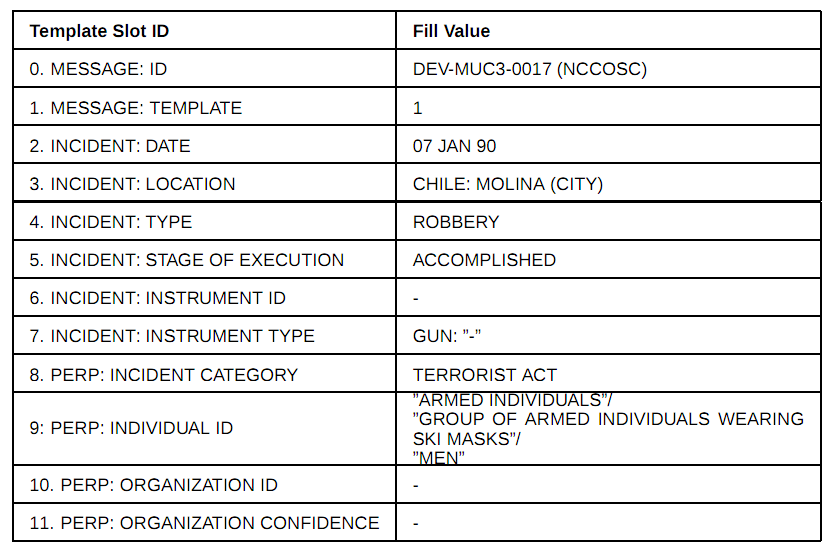
\includegraphics[scale=0.3]{template1.png}
\end{center}
\end{frame}

\begin{frame}
\frametitle{Information Extraction - Ejemplo}
\begin{center}
 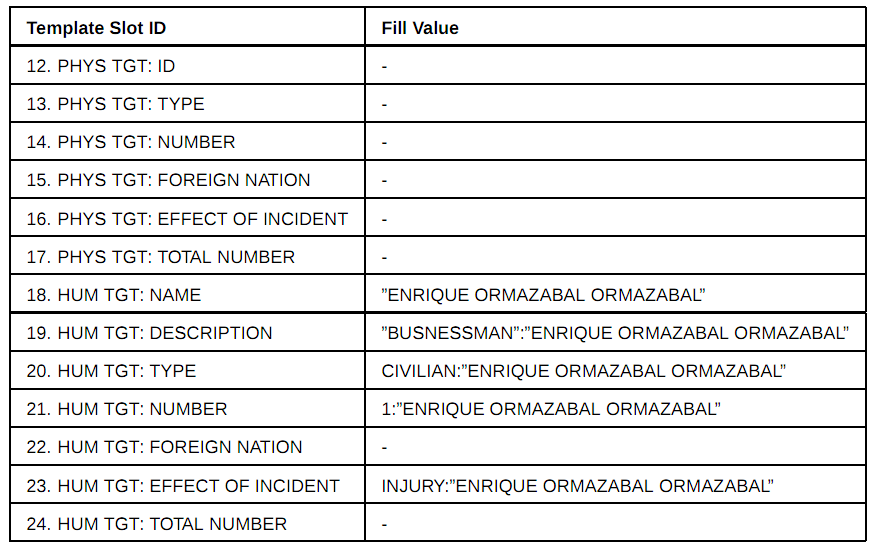
\includegraphics[scale=0.3]{template2.png}
\end{center}
\end{frame}

\begin{frame}
\frametitle{Information Extraction - Tipos de Tareas}
\begin{itemize}
 \item \textbf{Named Entity Recognition}: Identificación y extracción de nombres propios.
 \item \textbf{Template Element Task}: "Creación" de un template para características de un ente específico.
 \item \textbf{Template Relation Task}: "Creación" de un template para relaciones entre varios entes.
 \item \textbf{Coreference}: Capturar información de expresiones correferentes.
 \item \textbf{Scenario Template Task}: Son los ejemplos de la "vida real". Se pretende llenar un formulario con la información asociada a un evento, hecho o cualquier información estructurable.
\end{itemize}
\end{frame}

\begin{frame}
\frametitle{Information Extraction - Estructura}

\begin{center}
\begin{itemize}
 \item \textbf{Estructura de un Sistema de IE}
\end{itemize}
 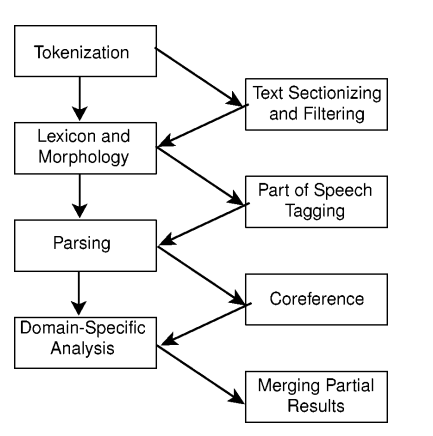
\includegraphics[scale=0.35]{estructura.png}
\end{center}

\end{frame}

\begin{frame}
\frametitle{Information Extraction - Aplicaciones}
\begin{itemize}
 \item Poblar una base de datos a partir de información de textos.
	\begin{itemize}
	 \item Resultados de juegos de beisbol en el periódico.
	 \item Alianzas, compras y fusiones de empresas.
	 \item Ataques terroristas obtenidos de las noticias.
	 \item Generación de resúmenes (por temas) a partir de artículos.
	 \item Extracción de metadatos de páginas web.
	\end{itemize}
\end{itemize}
\end{frame}

%\begin{frame}
%\frametitle{IE - Desempeño de una tarea de IE}

%\begin{block}{}
%P = Máximo total de respuestas correctas\\
%C = Número de respuestas correctas\\
%I = Número de respuestas incorrectas\\
%O = Número de respuestas sobregeneradas\\
%\end{block}
%
%\begin{itemize}
% \item \emph{Recall} = $ C / P $
% \item \emph{Precision} = $ C / C + I + O $
%\end{itemize}
%\begin{tikzpicture}[remember picture,overlay]  
%  \node [xshift=-3cm,yshift=-7.5cm] at (current page.north east)
%    { 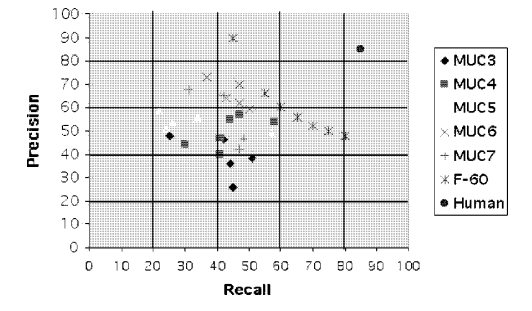
\includegraphics[scale=0.25]{rendimiento.png}};
%\end{tikzpicture}
%\end{frame}

\begin{frame}
\frametitle{Referencias}
\tiny{
\begin{itemize}
 \item D. Appelt. \emph{INTRODUCTION TO INFORMATION EXTRACTION} (http://philarts.spbu.ru/Members/lida\_pivovarova/Appelt.pdf)
 \item R. Grishman; B. Sundheim. \emph{MESSAGE UNDERSTANDING CONFERENCE 6: BRIEF HISTORY} (http://acl.ldc.upenn.edu/C/C96/C96-1079.pdf)
 \item OFFICIAL MUC 7 WEBPAGE (http://www.itl.nist.gov/iaui/894.02/related\_projects/muc/proceedings/muc\_7\_toc.html)
\end{itemize}
}
\end{frame}


\end{document}
